\chapter*{\textsc {Introduction}}
	\chaptermark{\textsc {Introduction}}

	\section{\textsc {Manipulation du TP}}
	
\paragraph{}	 
Le but de de cette manipulation est de réaliser un asservissement de niveau par retour de sortie. En effet, le vecteur d'état du procédé hydraulique n'est pas entièrement accessible par la mesure. On se propose ainsi de mettre en oeuvre l'estimation de l'état par un observateur.

\section{ \textsc{Présentation du système}}
\paragraph{}
Dans ce TP, nous utilisons le même procédé que celui utilisé dans le TP du module I4 intitulé "Modélisation, analyse et commande d'une distribution hydraulique à trois bacs d'eau". Voici, ci-dessous, les caractéristiques essentielles de la manipulation. On considère ici le procédé trois bacs :

\begin{figure}
\centering
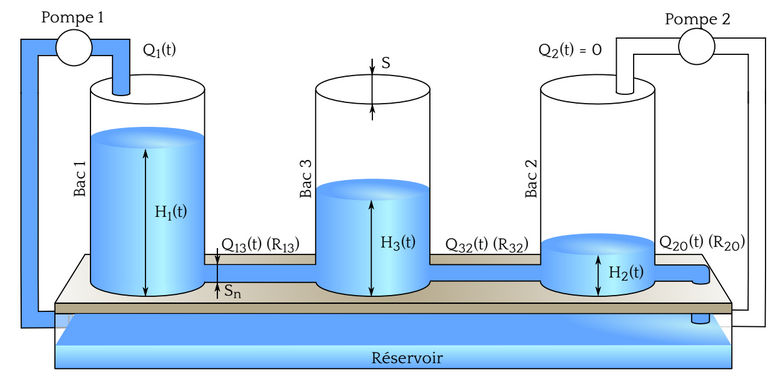
\includegraphics[scale = 0.5]{bac-deau.png}
\caption{Procédé trois bacs}
\label{fig11}
\end{figure}
 
 \paragraph{} La figure 1 représente le système du TP. Il est composé de trois bacs cylindriques en plexiglas de section S. Ces trois bacs sont disposés en série (de gauche à droite, on trouve les bacs 1, 3 et 2) et sont reliés par des tuyaux d'écoulement de section $S_n$.
\paragraph{} Le dernier bac 2 se vide par un cylindre, également de section $S_n$, dans le réservoir situé sous les trois bacs. Deux pompes de débit $Q_1(t)$ et $Q_2(t)$ permettent de remplir respectivement les bacs 1 et 3 avec l'eau récupérée dans le réservoir. Le système fonctionne donc ici en circuit fermé. 
\paragraph{} Les valeurs données par le constructeur sont $S=0,0154m^2$ et $S_n=5,10^{-5}m^2$. Les pompes obéissent à la relation $V_{qi}(t)=kQ_i(t)+b$, $i=1,2$. Avec $k=1,6.10^5$ et $b=-9.2592$. Où $V_{qi}(t)$ et $Q_i(t)$ représentent respectivement la tension appliquée à la pompe i et le débit correspondant.
\paragraph{} Les pompes sont alimentées par une tension comprise entre [-10V;10V]. Ainsi ke débit maximal, $Q_{max}$ délivré par une pompe est de $12.10^{-5}m^3/s$ lorsque la tension appliquée est de +10V. Les capteurs de niveau d'eau sont supposés linéaires autour du point de fonctionnement. Leur caractéristique est modélisé par l'équation $H_i(t)=k_iV_{h_i}(t)+b_i$, où $H_i$ est exprimé en mètres.

\section{\textsc{Le modèle linéarisé}}

\paragraph{} Nous considérons le procédé actionné par la seule pompe n1. Son débit $Q_1$ est compris entre [0,$Q_{max}$] suivant sa tension d'alimentation; le débit $Q_2$ délivré par la pompe 2 sera nul tout au long de la manipulation. Ainsi, les différentes hauteurs $H_1(t)$, $H_2(t)$ et $H_3(t)$ respectent par conséquent la condition $H_1(t)\ge H_3(t)\ge H_2(t)$. La seule mesure disponible lors de cette manipulation est la mesure de la hauteur d'eau $H_1(t)$.
\paragraph{} Le travail sera effectué sur un modèle aux faibles variations autou d'un point d'équilibre $H_0$ et un débit $Q_{10}$ à ce point d'équilibre de telle sorte que :\\

\begin{equation*}
\left\lbrace
\begin{array}{ccc}
Q_1(t) = q_1(t)+Q_{10} \\
H_1(t) = h_1(t)+H_{10}. \\
H_3(t) = h_3(t)+H_{30}. \\
H_2(t) = h_2(t)+H_{20}
\end{array}\right.
\end{equation*}
 
Avec $H_0 = [H_{10}~~H_{20}~~H_{30}]^T$ et $Q_{10}=3,5.10^{-5}$.\\

Les variations de hauteurs $h_1$, $h_2$ et $h_3$  vérifient la condition suivante :
$$h_1(t) \ge h_3(t) \ge h_2(t)$$.\\

En rappelant que la sortie mesurée est la hauteur d'eau $H_1(t)$, ce qui permet d'obtenir la variation de hauteur d'eau $h_1(t)$. Le modèle d'état linéarisé autour du point d'équilibre du procédé est donné par :

\begin{figure}
\centering
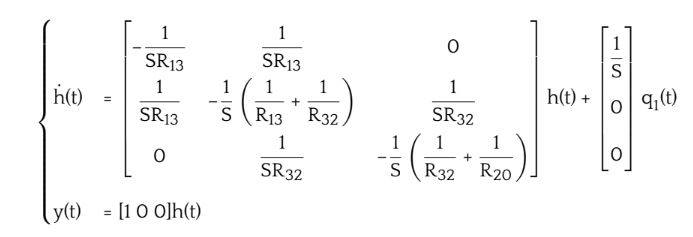
\includegraphics[scale = 0.5]{modele_detat_linearise.jpg}
\label{fig12}
\end{figure}

\paragraph{} Avec $h(t)=[h_1(t)~~h_2(t)~~h_3(t)]$. De manière conventionnelle, les matrices dynamique de commande et d'observation seront notées A, B et C. 
\paragraph{} On rappelle que $R_{ij}$ représente la résistance à l'écoulement dans les tuyaux reliant les bacs i et j :\large
$$R_{ij}=\frac{2\sqrt{|H_{i0}-H_{j0}|}}{a_{ij}}$$\normalsize
\paragraph{} Avec les trois coefficients d'écoulement : $a_{13}=0,4753S_n\sqrt{2g}$, $a_{32}=0,4833S_n\sqrt{2g}$ et $a_{20}=0,9142S_n\sqrt{2g}$.

